\chapter{Resultados e Discussão}

\section{Introdução} 

Neste capítulo, será abordado a sequência de testes realizados para o treinamento da RNC, assim como os resultados obtidos. Além disso, será apresentado a eficiência da utilização dos pesos da configuração de treinamento da YOLO que obteve a melhor performance. 

\section{Avaliação do Treinamento} 

Os resultados de desempenho obtidos das RNC, foram estruturados da seguinte forma: realização de uma avaliação do mAP, mAP50, mAP50-95 e recall das versões YOLOv5, YOLOv6 e YOLOv7, com variação do batch de 2 a 16, utilizando o otimizador SGD. Seguido, será avaliado o desempenho da YOLOv8, também com alteração de batch de 2 a 16, e com variação do otimizador. Por fim, será avaliado a performance na identificação de equipamentos, a partir de um conjunto de fotos não treinadas, e avaliar na prática a precisão real de cada configuração dos modelos, aplicadas. 

Foi discutido na Fundamentação Teórica deste trabalho que a YOLOv8 foi proposta como um modelo superior a suas três últimas versões. Em seu artigo de apresentação, foi comparado a taxa de sucesso da versão 8 contra a versão 5, 6 e 7, quando aplicado a um conjunto de imagens comuns \cite{ultralytics2023yolo}. Por isso, foi realizada a mesma experimentação, a fim de comparar, na configuração padrão de todos hiperparâmetros, se a escolha da oitava versão de fato mostra-se vantajosa. Apenas os parâmetros do batch foram alterados, a fim de verificar o efeito dos lotes no treinamento, conforme também realizado no estudo de \cite{gonzaga2023identificaccao}.

Por isso, por configuração padrão da rede neural YOLO, entende-se a utilização do otimizador SGD; com a taxa de aprendizado de 0,01; e configuração padrão de entrada das imagens de 640x640. 

\subsection{Resultados e análise do treinamento com a YOLOv5}

Na Tabela \ref{tab:yolov5-teste}, apresenta-se o resultado da aplicação da YOLOv5 ao dataset de reatores de núcleo de ar, alterando o valor de batch de 2 a 16. Nela, é evidente notar a primeira característica marcante de se diminuir o tamanho do batch: há um aumento no tempo de processamento da RNC, uma vez que lotes menores de imagens estão sendo analisados em cada iteração, demandam maior tempo para cobrir todo o escopo do dataset. No treinamento com a arquitetura YOLOv5, a mAP50 apresenta valores que podem ser considerados altos, inclusive maiores que aqueles apresentados no estudo de \cite{wang2023uav}, que também se dispôs a buscar modelos que identificassem objetos por meio de fotos obtidas de VANTs.

De modo geral, nesse sugere que o aumento do tamanho do batch de 2 para 8 resulta em melhorias significativas na precisão, recall, mAP50 e mAP50-95, ao mesmo tempo em que reduz o tempo de treinamento. No entanto, ao aumentar o batch size para 16, embora a precisão atinja seu valor mais alto, o recall e mAP50-95 apresentam uma pequena queda. Portanto, um batch size de 8 parece ser o mais eficiente em termos de equilíbrio entre desempenho e tempo de treinamento para este dataset específico.

\begin{table}[!hbt]
    \centering
    \begin{tabular}{|c|c|c|c|c|c|}
    \hline
    \multicolumn{6}{|c|}{\textbf{Otimizador SGD}} \\ \hline
    \textbf{Batch Size} & \textbf{Precisão} & \textbf{Recall} & \textbf{mAP50} & \textbf{mAP50-95} & \textbf{Tempo} \\ \hline
    2                   & 88.724                & 87.456               & 88.785              & 49.821                 & 48.75h             \\ \hline
    4                   & 89.831                 & 89.707               & 95.044             & 55.908                & 37.67h             \\ \hline
    8                   & 92.416                 & 91.922               & 96.197              & 60.488                 & 33.46h             \\ \hline
    16                  & 93.340                 & 90.977               & 95.474              & 54.689                 & 29.53h             \\ \hline
    \end{tabular}
    \caption{Resultados de diferentes tamanhos de batch aplicando YOLOv5}
    \label{tab:yolov5-teste}
\end{table}

\begin{figure}[!h]
    \centering
    \begin{minipage}{1\linewidth}
    \centering
    \captionsetup{justification=centering,margin=0.5cm,font=small}
    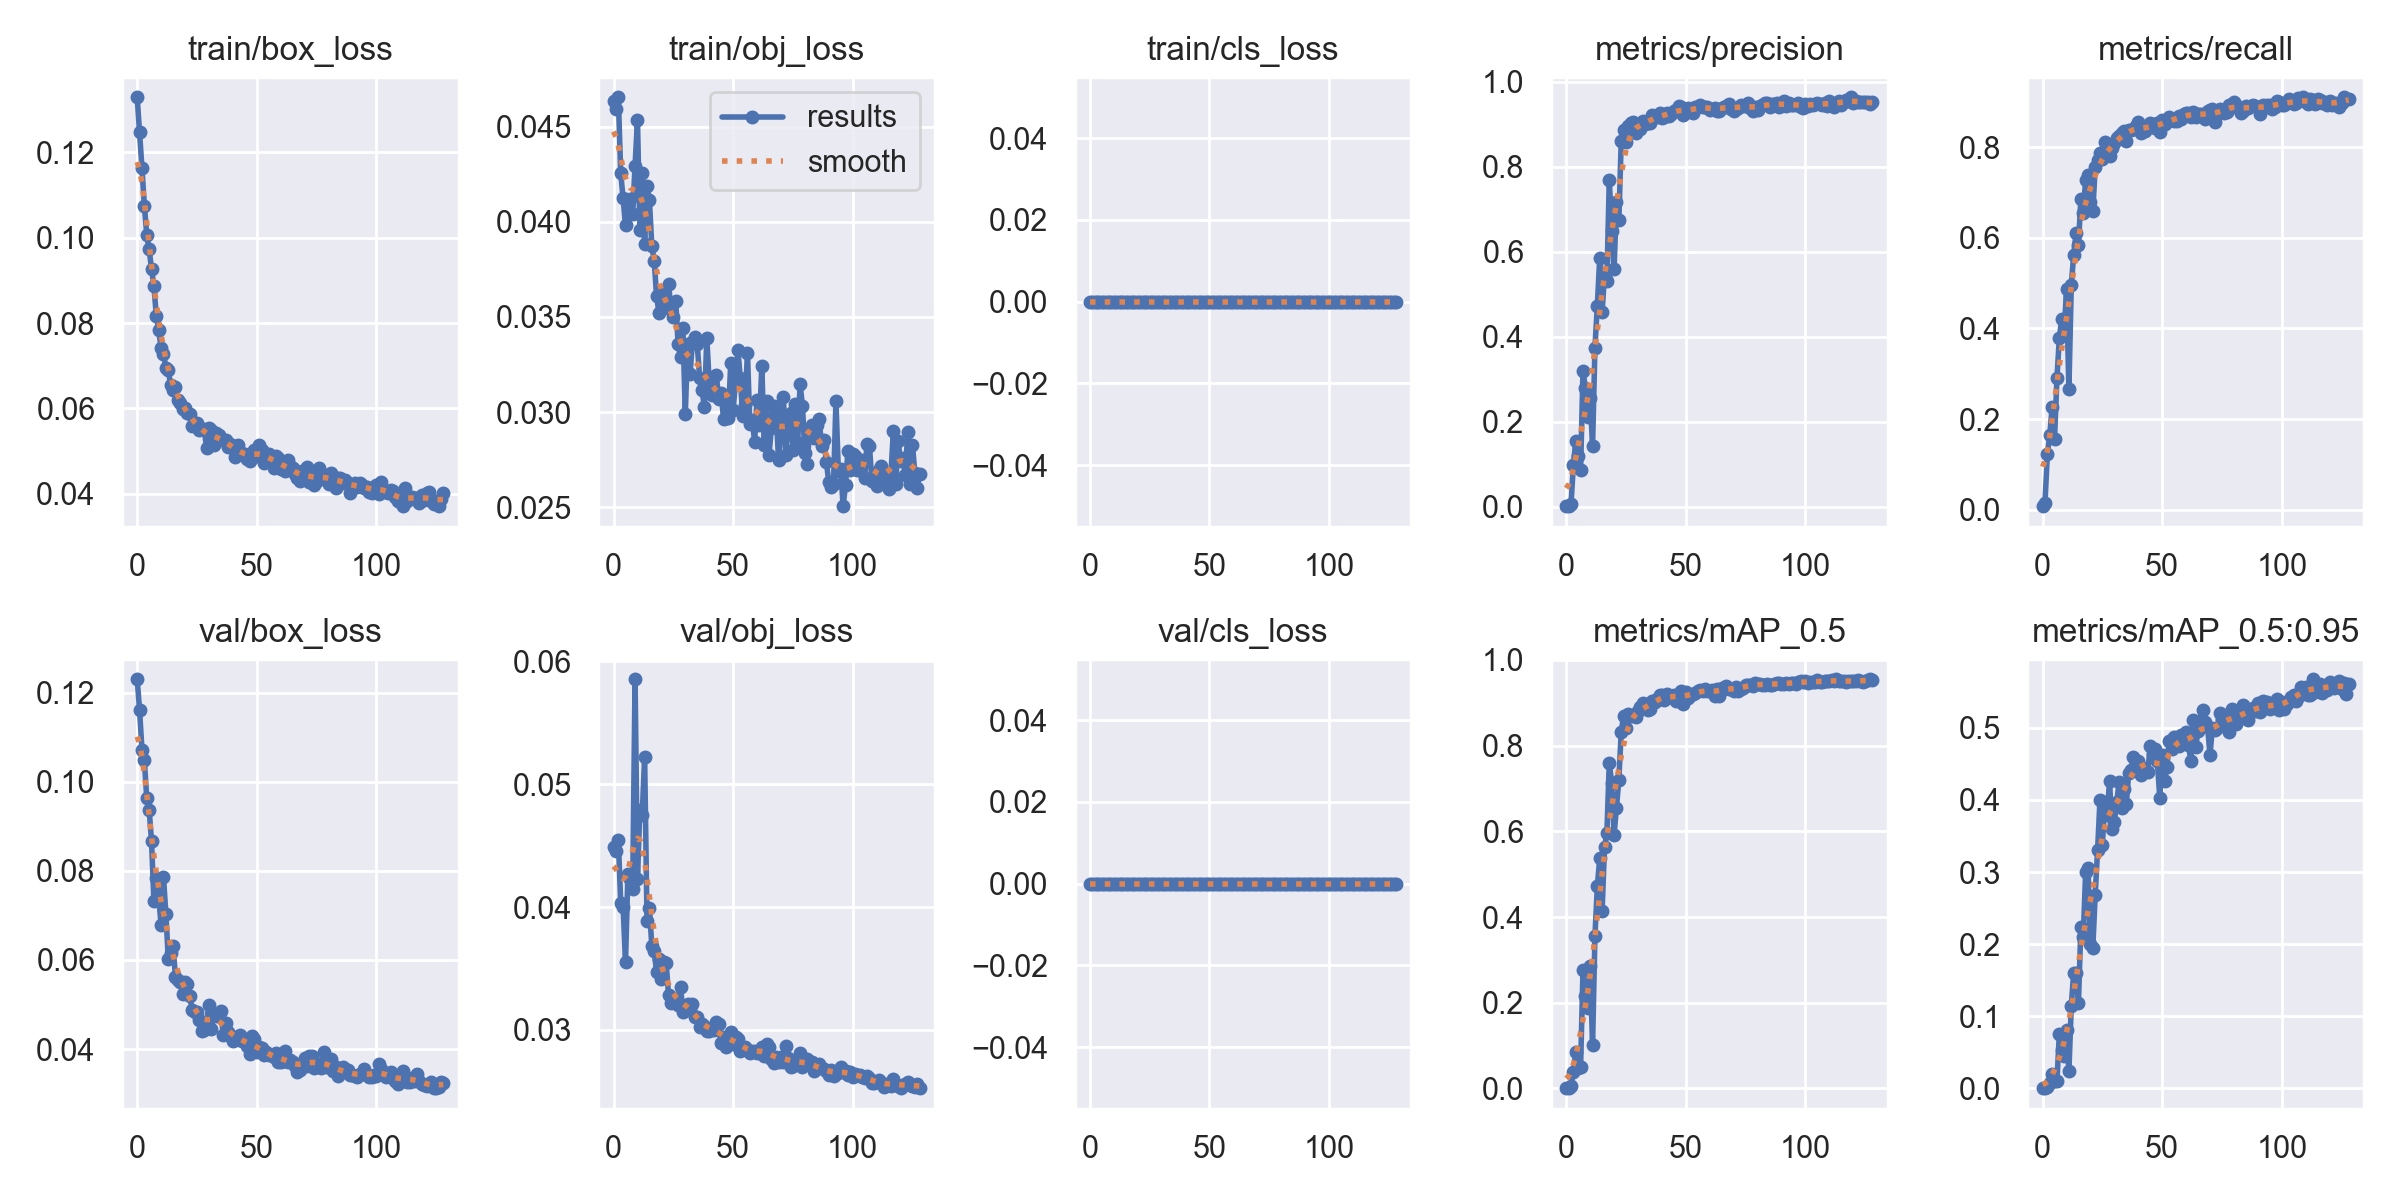
\includegraphics[width=1\linewidth]{img/cap6/results-yolov5-batch-16.png}
    \caption{Gráficos gerados a partir do treinamento com a YOLOv5, utilizando \textit{batch} igual a 16. Nota-se a evolução repentina para uma precisão acima de 90\%}.
    \label{fig:yolov5batch16}
    \end{minipage}
\end{figure}


\subsection{Resultados e análise do treinamento com a YOLOv6}

Embora a YOLOv6 tenha oferecido um leve aumento no recall em comparação com a YOLOv5, ela não trouxe melhorias significativas no mAP50-95, que permaneceu na casa dos 50\%. A precisão geral foi similar à YOLOv5, mas com uma pequena vantagem no batch size 16. A maior diferença foi observada no tempo de treinamento, que foi reduzido em todas as configurações, tornando a YOLOv6 mais eficiente em termos de tempo (Tabela \ref{tab:yolov6-teste}).

\begin{table}[!hbt]
    \centering
    \begin{tabular}{|c|c|c|c|c|c|}
    \hline
    \multicolumn{6}{|c|}{\textbf{Otimizador SGD}} \\ \hline
    \textbf{Batch Size} & \textbf{Precisão} & \textbf{Recall} & \textbf{mAP50} & \textbf{mAP50-95} & \textbf{Tempo} \\ \hline
    2                   & 88.523                & 86.225               & 87.895              & 50.705                 & 50.78h             \\ \hline
    4                   & 87.431                 & 90.505               & 94.124             & 54.108                & 39.85h             \\ \hline
    8                   & 91.578                 & 90.592               & 95.298              & 53.128                 & 32.65h             \\ \hline
    16                  & 92.775                & 92.332               & 94.548             & 56.739                 & 30.54h             \\ \hline
    \end{tabular}
    \caption{Resultados de diferentes tamanhos de batch aplicando YOLOv6}
    \label{tab:yolov6-teste}
\end{table}


\begin{figure}[!h]
    \centering
    \begin{minipage}{1\linewidth}
    \centering
    \captionsetup{justification=centering,margin=0.5cm,font=small}
    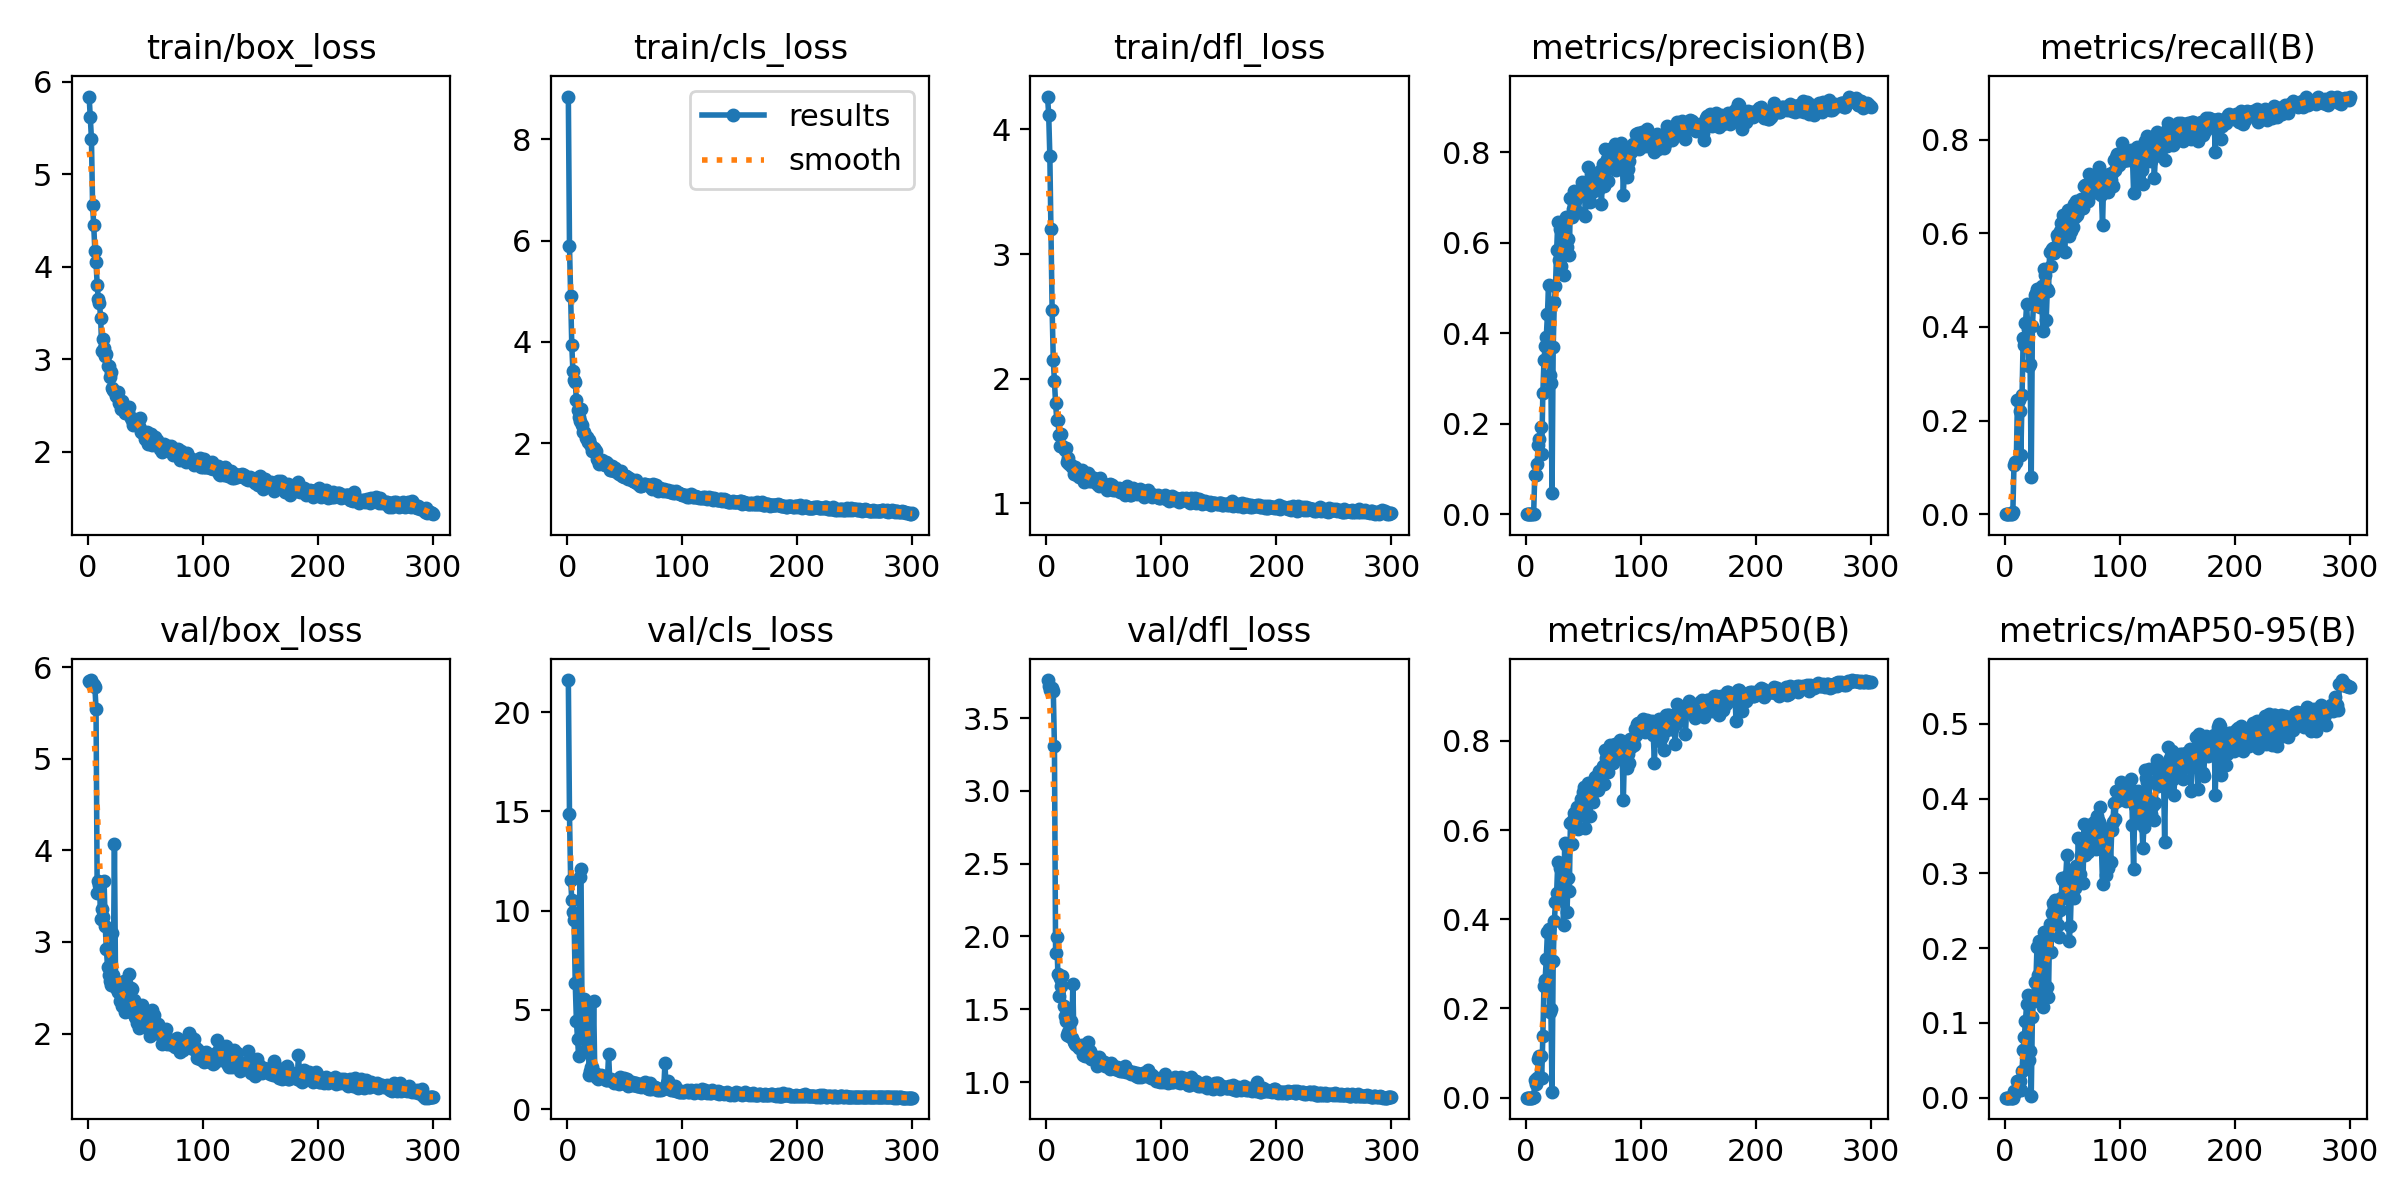
\includegraphics[width=1\linewidth]{img/cap6/results-yolov6-batch-16.png}
    \caption{Gráficos gerados a partir do treinamento com a YOLOv6.}
    \label{fig:yolov6batch16}
    \end{minipage}
\end{figure}


\subsection{Resultados e análise do treinamento com a YOLOv7}

A YOLOv7 apresentou variabilidade significativa nos resultados, com quedas notáveis na precisão e recall, especialmente para batch sizes menores. Embora tenha demonstrado estabilidade no tempo de treinamento, seu desempenho geral foi menos consistente em comparação com as versões anteriores. O mAP50-95, por exemplo, não superou os valores obtidos com a YOLOv5, sendo inclusive inferior em algumas configurações, como observado na Tabela \ref{tab:yolov7-teste}. Esta versão destacou-se pelo comportamento alternado, sugerindo um trade-off entre estabilidade temporal e eficácia.

\begin{table}[!hbt]
    \centering
    \begin{tabular}{|c|c|c|c|c|c|}
    \hline
    \multicolumn{6}{|c|}{\textbf{Otimizador SGD}} \\ \hline
    \textbf{Batch Size} & \textbf{Precisão} & \textbf{Recall} & \textbf{mAP50} & \textbf{mAP50-95} & \textbf{Tempo} \\ \hline
    2                   & 66.84                 & 59.45              & 62.42              & 53.45                 & 36.69h             \\ \hline
    4                   & 65.74                & 58.45               & 65.45            & 56.807                & 37.47h             \\ \hline
    8                   & 70.65                 & 59.582               & 68.57             & 54.71               & 38.46h             \\ \hline
    16                  & 73.11                 & 60.882               & 71.35               & 52.53                & 36.14h            \\ \hline
    \end{tabular}
    \caption{Resultados de diferentes tamanhos de batch aplicando YOLOv7}
    \label{tab:yolov7-teste}
\end{table}

\begin{figure}[!h]
    \centering
    \begin{minipage}{1\linewidth}
    \centering
    \captionsetup{justification=centering,margin=0.5cm,font=small}
    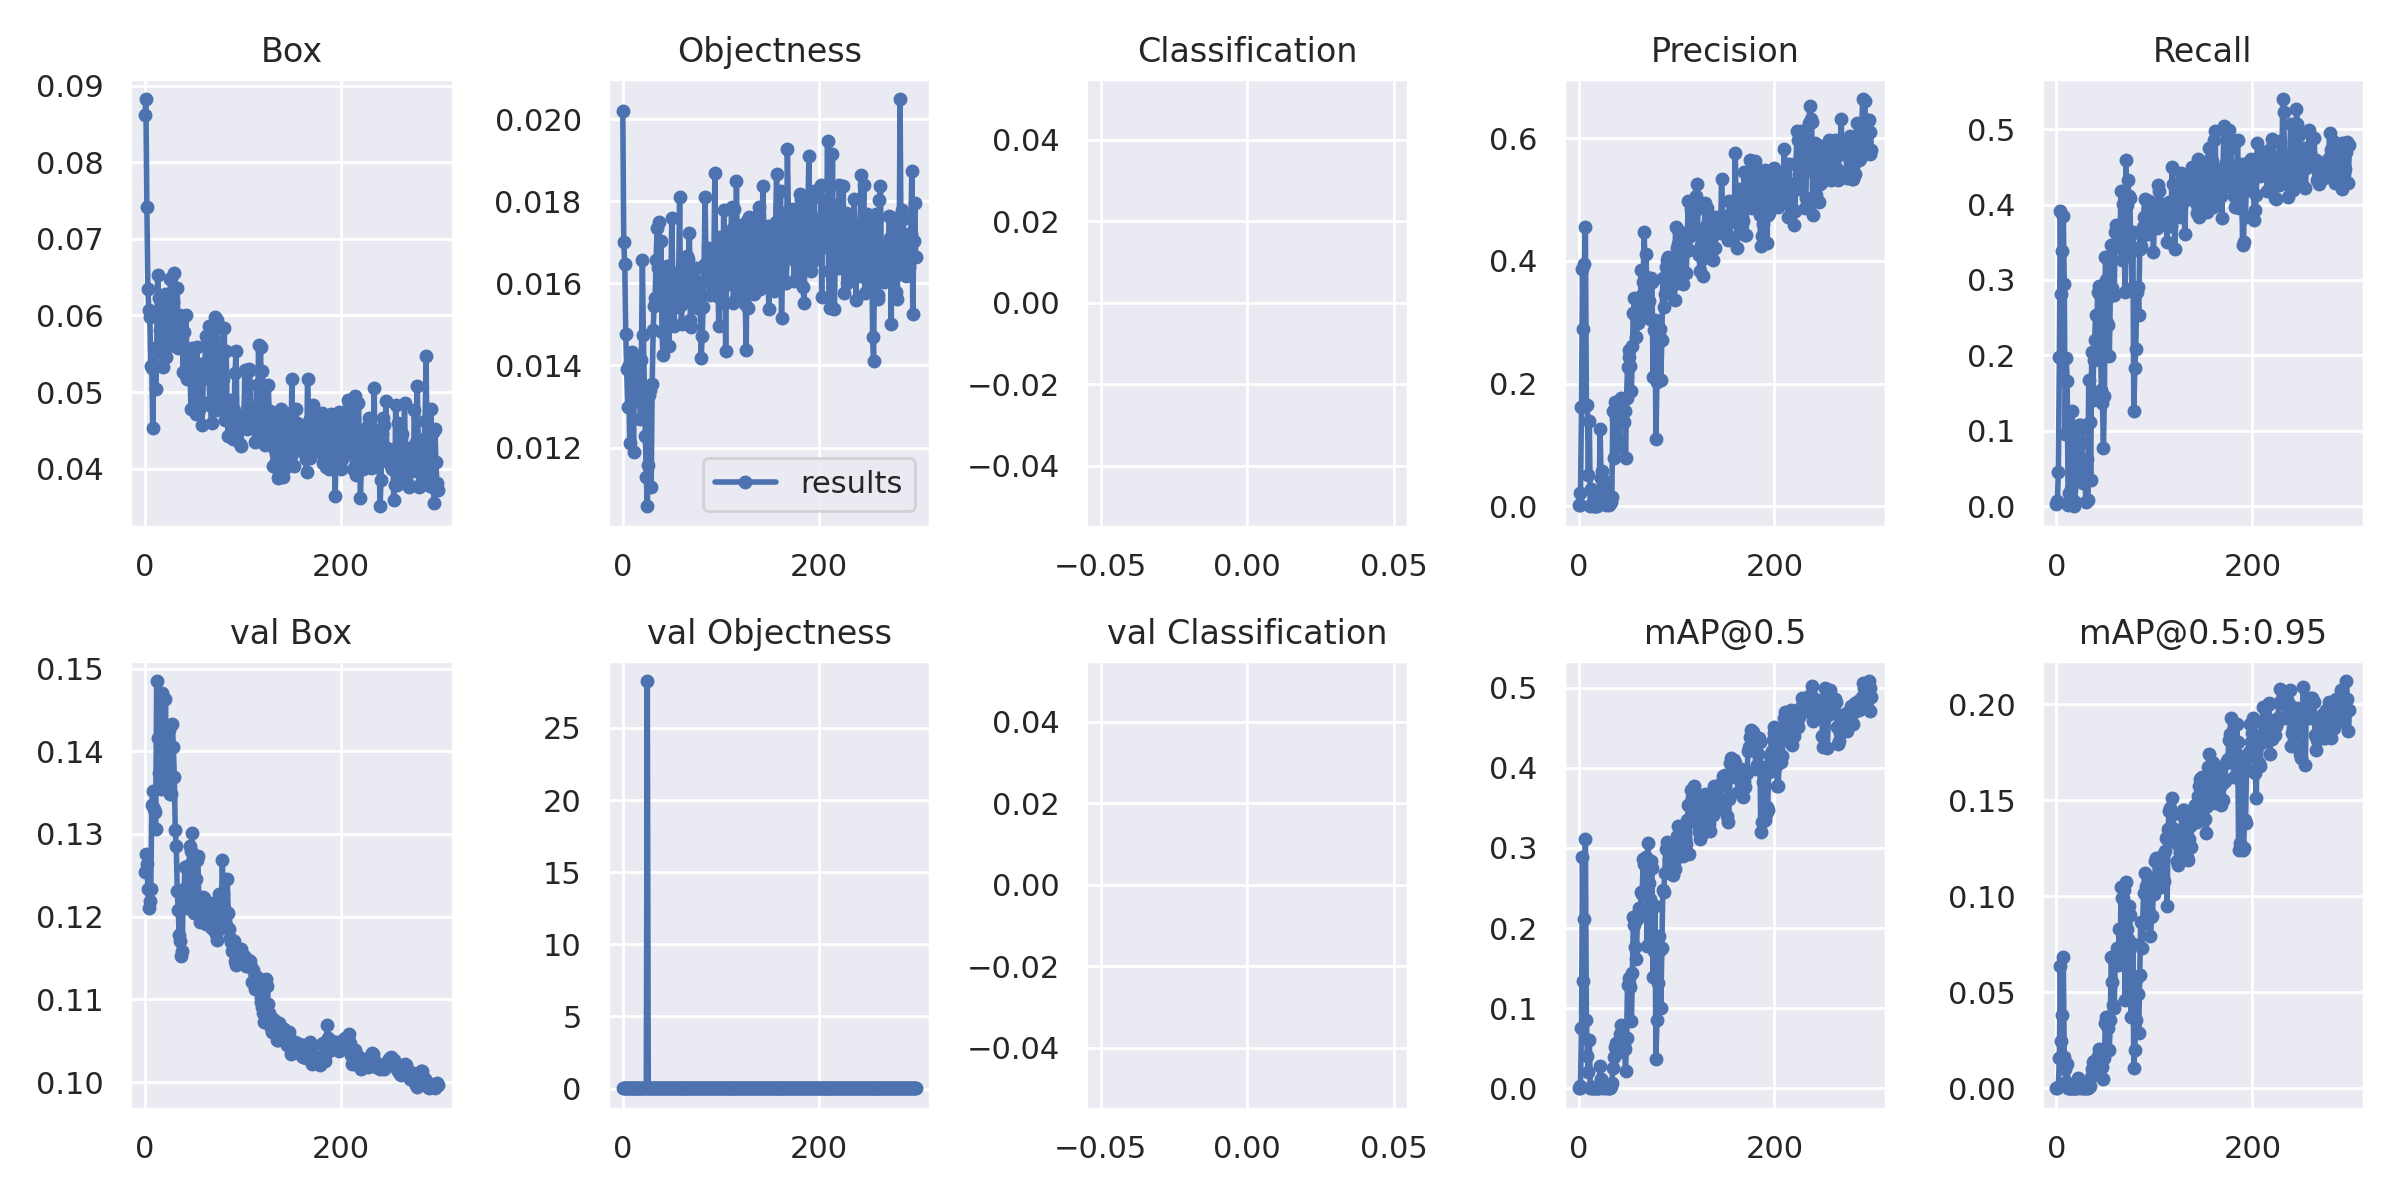
\includegraphics[width=1\linewidth]{img/cap6/results-yolov7-batch-16.png}
    \caption{Gráficos gerados a partir do treinamento com a YOLOv7, utilizando \textit{batch} igual a 16. O comportamento alternado sobressaltou-se nessa arquitetura}.
    \label{fig:yolov5batch16}
    \end{minipage}
\end{figure}

Comparando as três versões, a YOLOv5 mostrou-se superior em termos de desempenho geral, com alta precisão e mAP50-95, aliada a um tempo de treinamento eficiente. A YOLOv6, embora menos precisa, destacou-se pela redução do tempo de treinamento, sendo uma escolha viável quando a eficiência temporal é prioritária. Já a YOLOv7, apesar de sua estabilidade no tempo de treinamento, apresentou maior variabilidade nos resultados e um desempenho inferior em relação às versões anteriores, sugerindo que sua aplicação deve ser cuidadosamente considerada dependendo do contexto e das necessidades do projeto.

\subsection{Análise dos Resultados do Treinamento com YOLOv8}

Apresentou o melhor desempenho geral, destacando-se tanto em precisão quanto em recall, mAP50 e mAP50-95. A combinação com o otimizador AdamW se mostrou superior, oferecendo o melhor equilíbrio entre desempenho e tempo de treinamento, especialmente com batch size de 16

\begin{table}[!hbt]
    \centering
    \begin{tabular}{|c|c|c|c|c|c|}
    \hline
    \multicolumn{6}{|c|}{\textbf{Otimizador Adam}} \\ \hline
    \textbf{Batch Size} & \textbf{Precisão} & \textbf{Recall} & \textbf{mAP50} & \textbf{mAP50-95} & \textbf{Tempo} \\ \hline
    2                   & 91.323                       & 90.102                     & 94.022                     & 54.987                        & 33.071h                         \\ \hline
    4                   & 92.983                       & 91.857                     & 95.4                       & 57.704                        & 36.548h                         \\ \hline
    8                   & 92.383                       & 91.969                     & 95.006                     & 57.465                        & 31.221h                         \\ \hline
    16                  & 93.654                       & 92.964                     & 96.148                     & 60.269                        & 29.135h                         \\ \hline
    \end{tabular}
    \caption{Resultados de diferentes tamanhos de batch aplicando YOLOv8 e otimizador Adam}
    \label{tab:yolov8-adm}
\end{table}

A Tabela \ref{tab:yolov8-admw} mostra os resultados com o otimizador AdamW, onde a melhoria na precisão e no recall é ainda mais pronunciada. A precisão cresce de 93.886\% para 95.784\%, e o recall sobe de 91.954\% para 95.379\% com o aumento do tamanho do batch. As métricas de mAP50 e mAP50-95 atingem 97.858\% e 68.393\%, respectivamente, para o maior batch size. Embora o tempo de treinamento com AdamW seja consistente, o batch size de 16 proporciona o tempo mais reduzido de 28.013 horas, mostrando uma vantagem competitiva em relação ao Adam.

\begin{table}[!hbt]
    \centering
    \begin{tabular}{|c|c|c|c|c|c|}
    \hline
    \multicolumn{6}{|c|}{\textbf{Otimizador AdamW}} \\ \hline
    \textbf{Batch Size} & \textbf{Precisão} & \textbf{Recall} & \textbf{mAP50} & \textbf{mAP50-95} & \textbf{Tempo} \\ \hline
    2                   & 93.886            & 91.954          & 95.541         & 58.209            & 33.114h        \\ \hline
    4                   & 93.701            & 92.102          & 95.426         & 57.508            & 32.744h        \\ \hline
    8                   & 93.364            & 92.215          & 95.383         & 57.666            & 29.209h        \\ \hline
    16                  & 95.784            & 95.379          & 97.858         & 68.393            & 28.013h        \\ \hline
    \end{tabular}
    \caption{Resultados de diferentes tamanhos de batch aplicando YOLOv8 e otimizador AdamW}
    \label{tab:yolov8-admw}
\end{table}

Por fim, a Tabela \ref{tab:yolov8-sgd} apresenta os resultados com o otimizador SGD, que não só mostra uma melhoria contínua na precisão e no recall, com valores de 96.480\% e 94.718\% para o maior batch size, como também possui os melhores tempos de treinamento. O mAP50 e o mAP50-95 atingem 97.891\% e 68.245\%, respectivamente. O SGD combina o melhor desempenho em termos de métricas com a eficiência de tempo de treinamento, atingindo 27.633 horas para o maior batch size.

\begin{table}[!hbt]
    \centering
    \begin{tabular}{|c|c|c|c|c|c|}
    \hline
    \multicolumn{6}{|c|}{\textbf{Otimizador SGD}} \\ \hline
    \textbf{Batch Size} & \textbf{Precisão} & \textbf{Recall} & \textbf{mAP50} & \textbf{mAP50-95} & \textbf{Tempo} \\ \hline
    2                   & 94.466            & 93.062          & 96.421         & 61.710            & 35.448h        \\ \hline
    4                   & 94.989            & 93.779          & 96.759         & 65.201            & 31.018h        \\ \hline
    8                   & 95.618            & 94.621          & 97.123         & 66.451            & 29.787h        \\ \hline
    16                  & 96.480            & 94.718          & 97.891         & 68.245            & 27.633h        \\ \hline
    \end{tabular}
    \caption{Resultados de diferentes tamanhos de batch aplicando YOLOv8 e otimizador SGD}
    \label{tab:yolov8-sgd}
\end{table}

Em resumo, os dados indicam que aumentar o tamanho do batch geralmente melhora o desempenho do modelo em termos de precisão, recall e métricas de mAP, independentemente do otimizador utilizado. Entre os otimizadores testados, o SGD oferece o melhor equilíbrio entre desempenho e eficiência de tempo, seguido pelo AdamW, que proporciona alta precisão e recall, mas com um tempo de treinamento competitivo. O Adam, embora ainda eficaz, não alcança o mesmo nível de desempenho que os outros dois otimizadores. Esses resultados destacam a importância de escolher cuidadosamente o otimizador e o tamanho do batch para otimizar o treinamento e o desempenho do YOLOv8.

\subsection{Comparação de todas as versões}

Semelhante ao estudo de \cite{ultralytics2023yolo}, foi gerado um gráfico comparativo entre todas as versões da YOLO que aqui foram trabalhadas, tomando por base os resultados obtidos de mAP50-95 de cada, variando o tamanho de \textit{batch} nos valores de 2, 4, 8 e 16. Na Figura \ref{fig:compara-todas-yolo}, é apresentado o gráfico resultado da comparação. Nele, percebe-se visualmente que a YOLOv8, quando aplicada ao \textit{dataset} deste trabalho, se destaca com uma superioridade na precisão, em comparação com as três últimas versões, ratificando a proposta de seu uso. 

\begin{figure}[!h]
    \centering
    \begin{minipage}{0.7\linewidth}
    \centering
    \captionsetup{justification=centering,margin=0.5cm,font=small}
    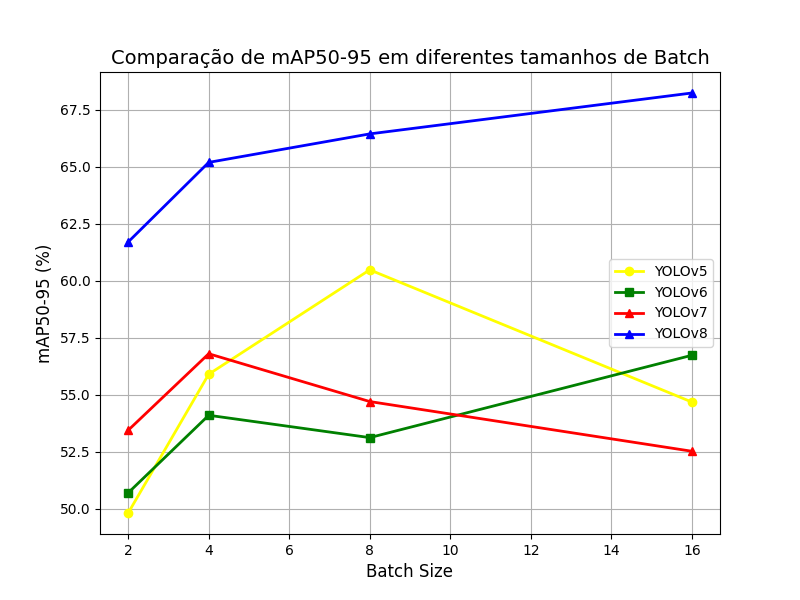
\includegraphics[width=1\linewidth]{img/cap6/comparacao-yolos-grafico.png}
    \caption{Comparação da YOLOv5 à YOLOv8, com otimizador SGD e variação de \textit{batch} de 2, 4, 8 e 16}.
    \label{fig:compara-todas-yolo}
    \end{minipage}
\end{figure}

As versões da YOLO não apresentaram um padrão claro de superioridade nem mostraram um crescimento consistente na precisão conforme o tamanho do \textit{batch} aumentava. Isso ocorre porque, ao serem expostas a diferentes tamanhos de \textit{batch}, as RNC podem não convergir de maneira previsível. A oscilação na precisão se deve às variações nos caminhos de aprendizado, que impactam os gradientes e tornam a otimização menos eficiente. Neste caso, tamanhos de \textit{batch} como 16, resultaram em um desempenho inferior para os modelos YOLOv5 e YOLOv7. Esse fenômeno pode ser atribuído à estagnação do aprendizado em regiões conhecidas como "planícies" ou \textit{plateaus}. Essas regiões são caracterizadas por uma diminuição na inclinação dos gradientes, levando a uma desaceleração no crescimento do aprendizado da RNC. Nessas situações, a rede pode se encontrar em um mínimo local, onde os ajustes dos pesos se tornam pouco eficazes, resultando em uma otimização subideal \cite{theorangeduck_minima_saddle}. Essa variabilidade no desempenho é uma característica comum em modelos de aprendizado profundo, especialmente em tarefas complexas como a detecção de objetos. A presença de planícies pode dificultar a exploração do espaço de parâmetros da rede, fazendo com que ela perca oportunidades de melhorar sua precisão \cite{goodfellow2016deep}.

A implementação do YOLOv8 com diferentes configurações de otimizadores e tamanhos de batch apresentou, no geral, resultados promissores, evidenciando uma tendência de melhora nas métricas conforme o aumento do tamanho do batch. Dentre as configurações avaliadas, a combinação do otimizador SGD com batch size de 16 se destacou por oferecer o melhor equilíbrio entre precisão, recall, mAP50, mAP50-95 e tempo de treinamento razoavelmente curto. Portanto, essa configuração específica, foi naturalmente escolhida para os testes subsequentes com o peso treinado.

\subsection{Avaliação da Implementação}

Na separação do conjunto de imagens para treinamento, foi adotada a prática de reservar 20\% do total de imagens para testes manuais. No caso, foram utilizadas 80 fotos para avaliar o desempenho do modelo treinado. A precisão média foi calculada aplicando o modelo em cada uma das 80 fotos, aferindo a quantidade de reatores detectados. A RNC apresentou resultados variados, identificando a quantidade exata de reatores em algumas imagens, enquanto em outras identificou um número superior ou inferior ao real. Para avaliar o desempenho, foi calculada a média absoluta da diferença entre os valores identificados e os valores reais presentes nas fotos, conforme a Equação \eqref{eq:media-identificacao}, em que \( R_{\text{e}} \) trata-se dos valores de reatores estimados pela RNC; enquanto \( R_{\text{p}} \), trata-se dos valoes presentes de reatores em cada imagem.

\begin{equation} \text{Média de Acertos da RNC} = \frac{1}{n} \sum_{i=1}^{n} \left(1 - \frac{|\text{R}{e_i} - \text{R}{p_i}|}{\text{R}_{p_i}}\right) \times 100\% \label{eq:media-identificacao} \end{equation}

Para avaliar a eficácia do modelo na prática, foram realizados testes com um conjunto de 80 imagens não vistas anteriormente. A Tabela \ref{tab:yolov8-eval} resume o desempenho do modelo YOLOv8 com a configuração ideal (SGD e batch size 16), revelando que 72,34375\% das imagens foram corretamente identificadas, refletindo uma taxa de acerto considerável. Conforme trabalho de \cite{barbado2022aplicaccao}, essa uma taxa de acerto para uma RNC acima de 70\%, para uma aplicação em nível de protótipo, mostra-se demasiada satisfatória. Com isso, o propósito do trabalho, que se coloca como uma proposição de utilização de uma tecnologia em evidência para melhora de um processo, é dado como atingido. 

\begin{table}[!hbt]
    \centering
    \begin{tabular}{|c|c|c|}
        \hline
        \textbf{Configuração} & \textbf{Número de Imagens Testadas} & \textbf{Taxa Média de Acerto} \\ \hline
        SGD + Batch Size 16 & 80 & 72,34375\% \\ \hline
    \end{tabular}
    \caption{Resumo do desempenho na aplicação da YOLOv8 na melhor configuração encontrada}
    \label{tab:yolov8-eval}
\end{table}

\section{Considerações Finais} 

O YOLOv8, como evolução natural das versões anteriores da família YOLO, traz melhorias significativas tanto na arquitetura do modelo quanto na eficiência do treinamento. Suas inovações permitem uma melhor detecção de objetos pequenos e maior precisão global, mantendo a rapidez e eficiência características dos modelos YOLO. A combinação de ajustes no tamanho do batch e a escolha do otimizador demonstram a flexibilidade do YOLOv8, permitindo sua adaptação a diversos cenários de aplicação, desde ambientes de baixa capacidade computacional até sistemas de alta demanda.

\begin{table}[!hbt]
    \centering
    \caption{Resumo comparativo dos trabalhos relacionados}
    \begin{tabular}{ >{\centering\arraybackslash}m{5cm} | >{\centering\arraybackslash}m{2cm} | >{\centering\arraybackslash}m{2cm} | >{\centering\arraybackslash}m{2cm} | >{\centering\arraybackslash}m{2cm} | >{\centering\arraybackslash}m{2cm} }
    \hline
    \cellcolor[gray]{0.9} \textbf{Trabalhos Relacionados} & 
    \cellcolor[gray]{0.9} \begin{sideways} \textbf{Alteração de Parâmetros da RNC} \end{sideways} & 
    \cellcolor[gray]{0.9} \begin{sideways} \textbf{Treinamento utilizando YOLOv8} \end{sideways} & 
    \cellcolor[gray]{0.9} \begin{sideways} \textbf{Utilização de VANT} \end{sideways} & 
    \cellcolor[gray]{0.9} \begin{sideways} \textbf{Subestações de Energia} \end{sideways} &
    \cellcolor[gray]{0.9} \begin{sideways} \textbf{Automação de Inserção de RV} \end{sideways} \\
    \hline 
    \cite{gonzaga2023identificaccao} & \textcolor{green}{\(\checkmark\)} & \textcolor{green}{\(\checkmark\)} & \textcolor{red}{\(\times\)} & \textcolor{red}{\(\times\)} & \textcolor{red}{\(\times\)} \\
    \hline
    \cite{diascomparaccao} & \textcolor{green}{\(\checkmark\)} & \textcolor{green}{\(\checkmark\)} & \textcolor{red}{\(\times\)} & \textcolor{red}{\(\times\)} & \textcolor{red}{\(\times\)} \\
    \hline
    \cite{wang2023uav} & \textcolor{green}{\(\checkmark\)} & \textcolor{green}{\(\checkmark\)} & \textcolor{green}{\(\checkmark\)} & \textcolor{red}{\(\times\)} & \textcolor{red}{\(\times\)} \\
    \hline
    (ZUZA et al. 2024) & \textcolor{green}{\(\checkmark\)} & \textcolor{green}{\(\checkmark\)} & \textcolor{green}{\(\checkmark\)} & \textcolor{green}{\(\checkmark\)} & \textcolor{green}{\(\checkmark\)} \\
    \end{tabular}
    \label{tab:relacionadoZuza}
\end{table}

Dessa forma, a escolha do SGD como otimizador, aliada a um tamanho de batch adequado, como o de 16, provou ser a configuração mais robusta para obter o equilíbrio ideal entre desempenho e custo computacional, tornando o YOLOv8 uma escolha vantajosa para aplicações de detecção de objetos, como os reatores de núcleo de ar, visando precisão e eficiência. Comparativamente, a Tabela \ref{tab:relacionadoZuza} faz o paralelo desta dissertação com os trabalhos correlatos apresentados no Capítulo 3, ressaltando os principais objetivos e motivos aqui trabalhados, confirmando que a proposta se mostrou bem sucedida.



